\documentclass[11pt,letterpaper]{article}
\usepackage{naaclhlt2013}
\usepackage{times}
\usepackage{amsmath}
\usepackage{graphicx}
\usepackage{latexsym}

\setlength\titlebox{6.5cm}    % Expanding the titlebox

\title{Instructions for NAACL HLT 2013 Proceedings\Thanks{This
    document has been adapted from the instructions for earlier ACL
    and NAACL proceedings, including those for 
    NAACL-HLT-12 by Nizar Habash and William Schuler,
    NAACL-HLT-10 by Claudia Leacock and Richard Wicentowski,
    NAACL-HLT-09 by Joakim Nivre and Noah Smith, 
    for ACL-05 by Hwee Tou Ng and Kemal Oflazer,
    for ACL-02 by Eugene Charniak and Dekang Lin, and earlier ACL and
    EACL formats.  Those versions were written by several people,
    including John Chen, Henry S. Thompson and Donald Walker.
    Additional elements were taken from the formatting instructions of
    the {\em International Joint Conference on Artificial Intelligence}.  
    This second version clarifies the procedure for 
    submitting for double-blind reviewing.}}

\author{Author 1\\
	    XYZ Company\\
	    111 Anywhere Street\\
	    Mytown, NY 10000, USA\\
	    {\tt author1@xyz.org}
	  \And
	Author 2\\
  	ABC University\\
  	900 Main Street\\
  	Ourcity, PQ, Canada A1A 1T2\\
  {\tt author2@abc.ca}}

\date{}

\begin{document}
\maketitle
\begin{abstract}
  This document contains the instructions for preparing a camera-ready
  manuscript for the proceedings of NAACL HLT 2013.  The document itself conforms
  to its own specifications, and is therefore an example of what
  your manuscript should look like.  Papers are required to conform to
  all the directions reported in this document.  Also included are instructions for
  submission to the conference, which are similar to the camera-ready instructions
  but remove author-identifying information.
\end{abstract}



\section{Introduction}
\label{ssec:intro}


\section{Experiment}
\label{ssec:exp}

We experiment with multiple dataset as the original paper\cite{DBLP:journals/corr/Johnson014} refers, specifically, we use the IMDB and Elec
dataset as benchmark. Our code and documentation is available for reproducing the result.

\subsection{CNN}
Here most of the parameters used in CNN is the same as the original paper shows, we use the fixed rectifier
$\sigma{(x)} = max(x, 0)$ and minimized square loss with $L_{2}$ regularization by \textit{stochastic gradient descent}
(SGD). Since we want to explore the ability of CNN layers as well as the BOW features, we modified the
structure definition, and tuned the parameters in new network structure.

In our experiment, for example, seq-CNN has a fixed region size of 3, and for bow-CNN, we add two convolutional
layers, with another additional bow feature layers that treat the whole document as one region, it has the fixed 20 neurons
in this layer. In bow-CNN, to avoid computational cost, we used a variable size of stride named \textit{p}, currently
we set it as 2 and 3, and the padding size is set to be \textit{p-1}. These parameters are essential for faster
convergence and strong representation. To explore better result, we did some experiments to adjust the size of stride,
for example, we want to add a new layer as convolutional layer, so we set another layer with stride size of 4, which means
that the first three layers are convolutional layers with stride size of 2, 3 and 4, and then combined with the bow feature
layers, to see if it helps for improving the accuracy. A detailed description about the result is show in the result
section. Other important parameters we adopted is the \textit{dropout}\cite{hinton2012improving} and \textit{response normalization}\cite{krizhevsky2012imagenet}, we use the
parameters by default as the same with the previous paper.

\subsection{Baseline}
For comparison, we use both the previous SVM method with linear kernel and the CNN method. Based on previous experiment, the
NB-LM which first appeared as NB-SVM, is the best result in WM12\cite{wang2012baselines}. This SVM method first generates the bag-of-$n$-gram
feature vectors, and then multiplies the components for each $n$-gram $f_{i}$ with $log(P(f_i|Y=1)/P(f_i|Y=-1))$(NB-weight).
The probability $P$ is estimated by the training data.

For the CNN-method, as the original shows, they have seq-CNN, bow-CNN, seq2-CNN and seq2-bow$n$-CNN. These four proposed methods are
better than the NB-LM method in most cases using IMDB, Elec and RCV1 dataset, as the Table~\ref{baseline-table} shows, due to
the proprietary of RCV1, we don't do experiment on this dataset. Our main target is to design a more advanced structure or feature
representation to better improve the accuracy, so we mainly compare our result with the best result using seq2-bow$n$-CNN 
as the bold number shows, but we will also conduct some experiment for comparison to show our hypothesis and proof.


\begin{table}
\begin{center}
\begin{tabular}{|l|r|r|c|}
\hline \bf methods & \bf IMDB & \bf Elec & \bf RCV1 \\ \hline
SVM bow3(30K) & 10.14 & 9.16 & 10.68 \\
SVM bow1(all) & 11.36 & 11.71 & 10.76 \\
SVM bow2(all) & 9.74 & 9.05 & 10.59 \\
SVM bow3(all) & 9.42 & 8.71 & 10.69 \\
NN bow3(all) & 9.17 & 8.48 & 10.67 \\
NB-LM bow3(all) & 8.13 & 8.11 & 13.97 \\
\hline bow-CNN  & 8.66 & 8.39 & 9.33 \\
seq-CNN & 8.39 & 7.64 & 9.96 \\
seq2-CNN & 8.04 & 7.48 & - \\
seq2-bow$n$-CNN & \textbf{7.67} & \textbf{7.14} & - \\
\hline
\end{tabular}
\end{center}
\caption{\label{baseline-table} Baseline method with error rate(\%). }
\end{table}


\subsection{Dataset}

{\bf IMDB: movie review} IMDB dataset provide a series of reviews that are
labelled as positive or negative, this dataset is mainly used for sentiment
analysis. The size is roughly 25K reviews, and we used them for training
and testing. There are only two classes(\textit{negative} or \textit{positive})
for all the reviews.


{\bf Elec: electronic product reviews} Elec is similar to the IMDB, they're part
of Amazon's product view with five-star range of grading, we choose the 1-2 star
as negative and 4-5 star as positive. The remaining steps are the same as IMDB,
before tagging we also tokenize and do some data preprocessing tasks.


{\bf RCV1: topic categorization} RCV1 is a corpus of Reuters news articles which
contains 103 topic categories. Each article may have multiple category labels.


There is no available test result in the original paper about seq2-bow$n$-CNN, which
is the state-of-art result and the dataset is not available for us to train and test. 
So we don't have baseline and training data for this dataset, and our design is 
mainly based on the previous two datasets, especially the IMDB dataset.

\subsection{Result}
\label{ssec:result}

We proposed several hypothesis and did some experiment to verify it. In this section,
we will give separate descriptions about our experiment.

\subsubsection{Increasing convolutional layers}

In the previous work, we can conclude that with increased convolutional layer, the error
rate will decrease no matter what database we use. For the Table~\ref{baseline-table}, we
can see that seq2-CNN is much better that seq-CNN, the error rate decrease from 8.39\% to
8.04\% in IMDB and from 7.64\% to 7.48\%.

Our hypothesis lays in the ground that with more convolutional layer, each layer contains
the feature that has different stride, we can obtain more word order information in the new
stride, and this information can exclude the possibility that only unigram, bigram and trigram
that have the influence on classification result. If the hypothesis works, we will tried more
layers with enhanced methods to cascade the improving direction.

To verify our result, we first increase the convolutional layer by 1, as the Figure~\ref{seq-CNN-figure}
shows.

\begin{figure}
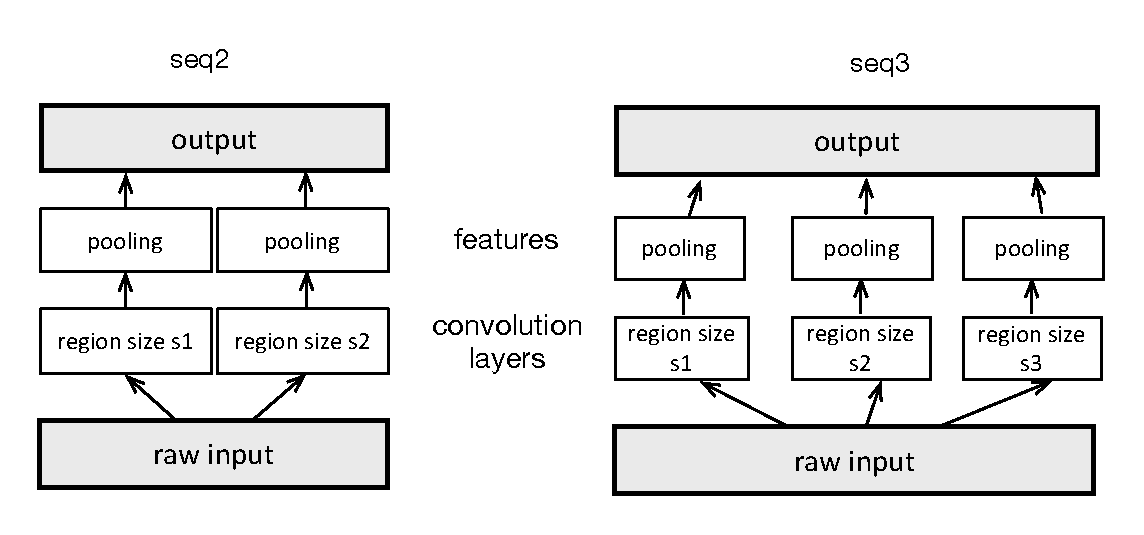
\includegraphics[width=3in]{seq2-CNN.eps}
\caption{\label{seq-CNN-figure} architecture in seq2 vs seq3}
\end{figure}

From the figure we can see that there is a new parallel convolutional layer and pooling layer, all the
results are merged into the output layer. The final result is shown in Table~\ref{conv-table}. From
the table we can see that the final accuracy is not essential in relation with the depth of convolutional
layers, even if we increase the convolutional layer depth, the result still doesn't beat the simple
seq2-CNN. We should note that to avoid the coincidence, the seq3-CNN is done multiple times and the average
rate is calculated as the final result. 

This experiment is done on GPU K40, with 6 GPUs and each GPU is
equipped with 12GB memory. It takes roughly 1 hour to finish one experiment if the GPU is available without
any tasks running on it. We don't use other more layers to experiment due to the limited resources and running
time, but it still gives us some directions to work on.

\begin{table}
\begin{center}
\begin{tabular}{|l|r|r|c|}
\hline \bf methods & \bf IMDB & \bf Elec & \bf RCV1 \\ \hline
NB-LM bow3(all) & 8.13 & 8.11 & 13.97 \\
\hline seq-CNN & 8.39 & 7.64 & 9.96 \\
seq2-CNN & 8.04 & 7.48 & - \\
seq3-CNN & \textbf{8.12} & - & - \\
\hline
\end{tabular}
\end{center}
\caption{\label{conv-table} error rate(\%) with different convolutional layers}
\end{table}

From this experiment, we can see that the representation or feature vector is not essentially in linear relation
with the depth of the convolutional layers. Two convolution layers seem to be the best practical configurations
for the text classification tasks here, especially for IMDB and Elec.


\subsubsection{Using more bow features}
Due to the failure of the first trial, we want to seek new feature representation. As the previous work shows,
NB-weight feature vector is quite useful before the occurrence of CNN. In their orignal paper, the error rate
is decreasing when using the bow n-gram features instead of convolutional layers. For example, the error rate
in IMDB decrease from 8.04\% to 7.67\%, and in Elec it's from 7.48\% to 7.14\%.

The difference between seq2-bow$n$-CNN and seq2-CNN is that it adds a brand new bow feature layer instead of
the convolutional layer, and this new bow feature can help to decrease the error no matter what the dataset it
is. Comparing with convolutional layer seq3-CNN, which uses the additional convolutional layer, not the bow$n$
feature layer in seq2-bow$n$-CNN, even though they have the same depth, seq2-bow$n$-CNN is still much better
than convolutional layer CNN.

\begin{figure}
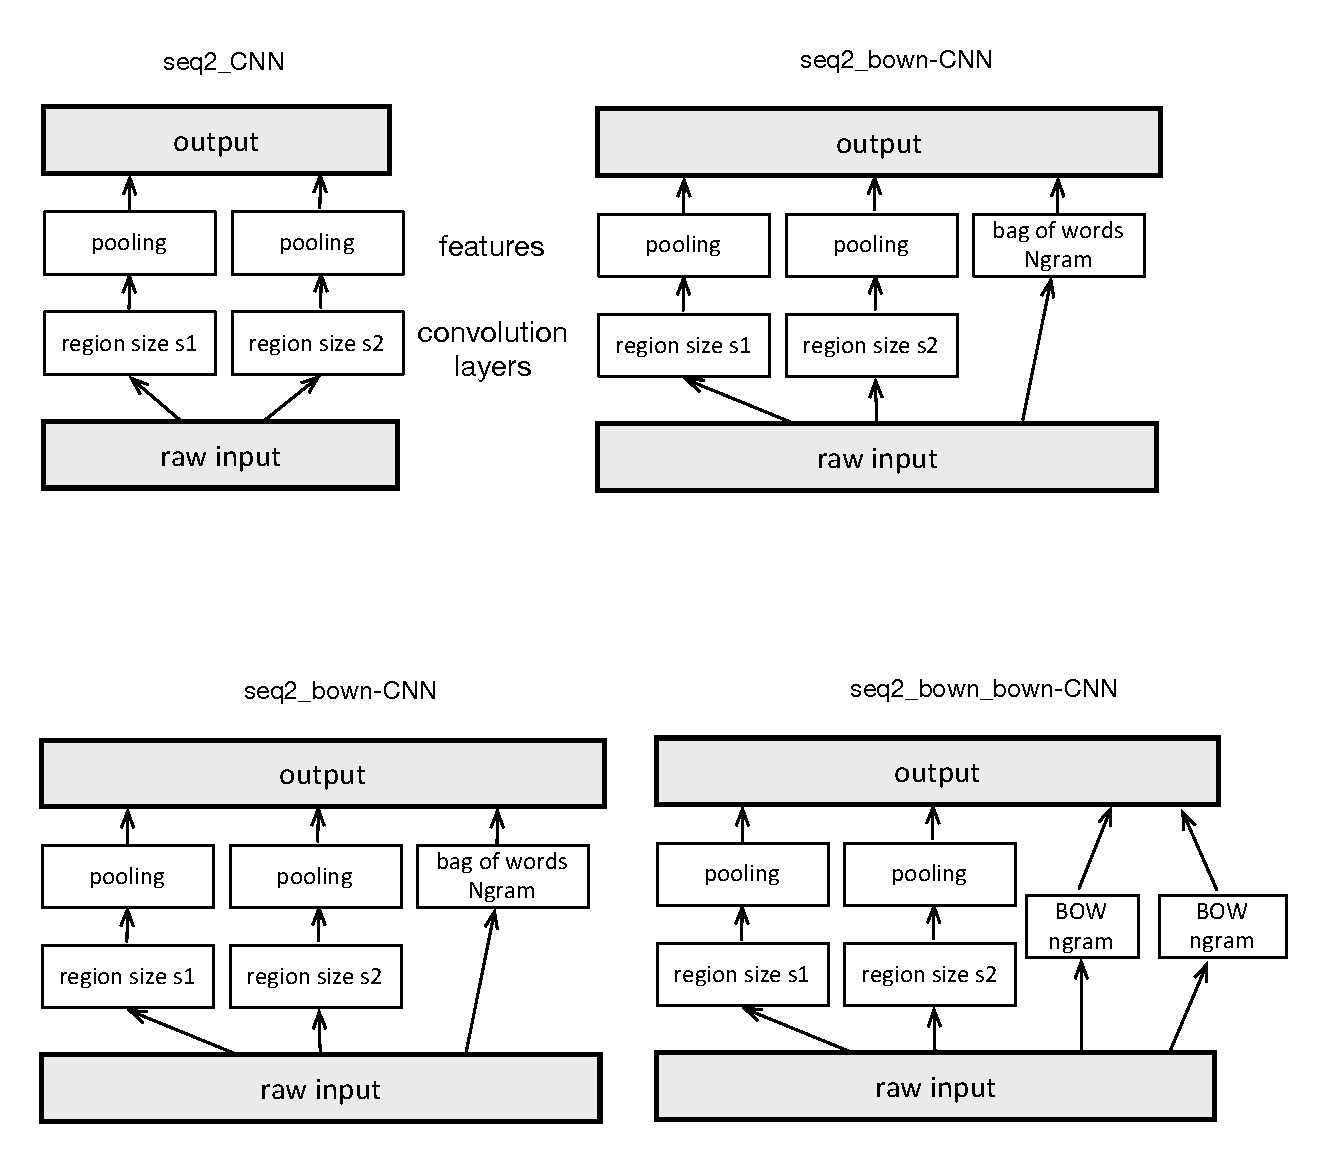
\includegraphics[width=3in]{seq-bown-CNN.eps}
\caption{\label{bown-CNN-figure} seq-CNN vs bown-CNN}
\end{figure}


Inspired by this observation, we guess that adding new bow $n$-gram feature layer should contribute to the
improvement of the accuracy. What if we increase a new bow $n$-gram feature? The last seq2-bow$n$-bow$n$-CNN
is our design for this specific task. By adding a new bow $n$-gram feature layer, we think the error rate should
be decreased by some degree.

\begin{table}
\begin{tabular}{|l|r|r|c|}
\hline \bf methods & \bf IMDB & \bf Elec & \bf RCV1 \\ \hline
NB-LM bow3(all) & 8.13 & 8.11 & 13.97 \\
\hline bow-CNN  & 8.66 & 8.39 & 9.33 \\
seq-CNN & 8.39 & 7.64 & 9.96 \\
\hline seq2-CNN & 8.04 & 7.48 & - \\
seq2-bow$n$-CNN & \textbf{7.67} & \textbf{7.14} & - \\
seq2-bow$n$-bow$n$-CNN & \textbf{7.72} & - & - \\
\hline seq3-CNN & \textbf{8.12} & - & - \\
\hline
\end{tabular}
\caption{\label{bow-table} error rate(\%) with bow$n$ features}
\end{table} 


The final result is shown in Table~\ref{bow-table}. From the table we can see that without convolutional layer,
bow is still worse that CNN(bow-CNN vs seq-CNN), but under the basis of two convolutional layer(seq2), using additional
bow$n$ feature layer contributes to the overall classification. Our new seq2-bow{n}2-CNN use another additional $n$-gram
feature layer. To utilize the word order, the new bow feature should has different vector from the previous layer, so we
use 4-gram, 5-gram ,6-gram as the input of bow feature vectors. By combining the two bow feature layer, 
with the previous two convolutional layers, we proposed our new architecture. In the final step, we run the experiment 10
times and get the average value of the error rate, it's 7.72\%, which is quite close to the state-of-art error rate 6.67\%,
but it still much better than the previous seq3-CNN.

Even though we don't get much better result than expected, the result shows that adding new bow feature layer will not harm
the overall accuracy significantly, and comparing with other previous experiment, we can conclude that bow feature layer
actually is better than convolutional layer, under the basis of several convolutional layers existed before.


\subsubsection{Using more grams}
After the first two trials, we get some useful conclusions and results, but it still didn't improve the result significantly,
and our hypothesis seems not working well under some constrain of the low dimension CNN feature. We explored a lot of modification
of the network structure as well as the sampling schema. However, we can get to know the bow feature is quite useful comparing
with convolutional feature, and if we can get a better representation of the feature vectors, then we can have a stronger
representation of the texts.

Based on the above assumption, we want to improve the features of the bow vectors. Before we use the unigram, bigram and trigram
as the input of the NB-weight, then we used these weights to generate bow features, as the bow feature layer. However, by a bold
assumption, maybe using more grams will yield a better representation. As we learned from the class that Google has used at most
6-gram, so why not trying to add more grams as the input to generate a better bow feature?

By this assumption, we modified the code to allow for more grams instead of the fixed unigram, bigram and trigrams. After the union
of these grams with 4-gram, the overall grams are the input of the bow features.

\begin{table}
\begin{tabular}{|l|r|r|c|}
\hline \bf methods & \bf IMDB & \bf Elec & \bf RCV1 \\ \hline
NB-LM bow3(all) & 8.13 & 8.11 & 13.97 \\
\hline seq2-bow$n$-CNN & \textbf{7.67} & \textbf{7.14} & - \\
\hline seq2-bow$n$-4CNN & \textbf{7.48} & - & - \\
\hline
\end{tabular}
\caption{\label{bow4-table} error rate(\%) with 4-gram bow}
\end{table} 

From the new Table~\ref{bow4-table}, we can see that our newest error rate is 7.48\%, which is lower than the state-of-art error rate. Even though
it only decrease 0.2\%, it's still a big increase as their original work only improve the NB-LM by 0.5\%, our work push their work
forward and give a more lower error rate. And it also open a path for the future direction.


\subsection{Discussion}

From the above experiment, we have made some good progress for better seq-bow$n$-CNN features, using this new feature with its corresponding parameters, we can achieve the lowest error rate. By analyzing the three explorations of our experiment, we can see bow is better than the
convolutional layer. Even though we can achieve a higher accuracy with two convolutional layer, it doesn't mean that this can work well for
more layers. Our explanation for this phenoment is that unlike image, the text doesn't convey so much spatial correlation and by using two
convolutional layers it's enough to represent the word order and utilize them in this simple structure is enough.

Apart from that, if we want to better improve, simply using the convolutional layer's feature is not enough. By using the previously state-of-art
NB-LM features, we get the idea of bow feature's strong ability in text categorization. So we combine the convolutional layer with the bow features,as the input of the final output layer, which gives a better accuracy. And based on the theory behind the NB-LM, we further improve the
bow features by using more grams, and it gives us an even better result. The final result shows that combing bow feature with convolutional neural
network's feature under the fine-tuned and well-defined network structure can give us the best result in text categorization tasks. In the future,
we can explore more on the optimization of these two areas and achieve an even better classifier.







\end{document}
